\noindent
La figura~\ref{fig:vista-cooperacion-aplicacion} muestra la vista de cooperación de aplicaciones, en la cual se representa la interacción entre los componentes de la arquitectura de virtualización y contenerización. En la capa de aplicaciones, se observa el entorno de Containers Applications, conformado por K3S, Containerd, Kubectl y los Pods, que trabajan en conjunto para la gestión y ejecución de contenedores. Estos elementos se relacionan con la infraestructura subyacente compuesta por el hipervisor, las \VM\ y los servicios de almacenamiento, los cuales habilitan los recursos. Asimismo, la red interna del \GRID\ actúa como medio de comunicación entre los distintos componentes, mientras que el \textit{firewall} ofrece un nivel de seguridad adicional al controlar los accesos. Esta vista evidencia la cooperación entre la capa de contenerización y la capa de infraestructura, permitiendo la integración de servicios de red, cómputo y seguridad en un ecosistema unificado.
\begin{figure}[H]
    \centering
    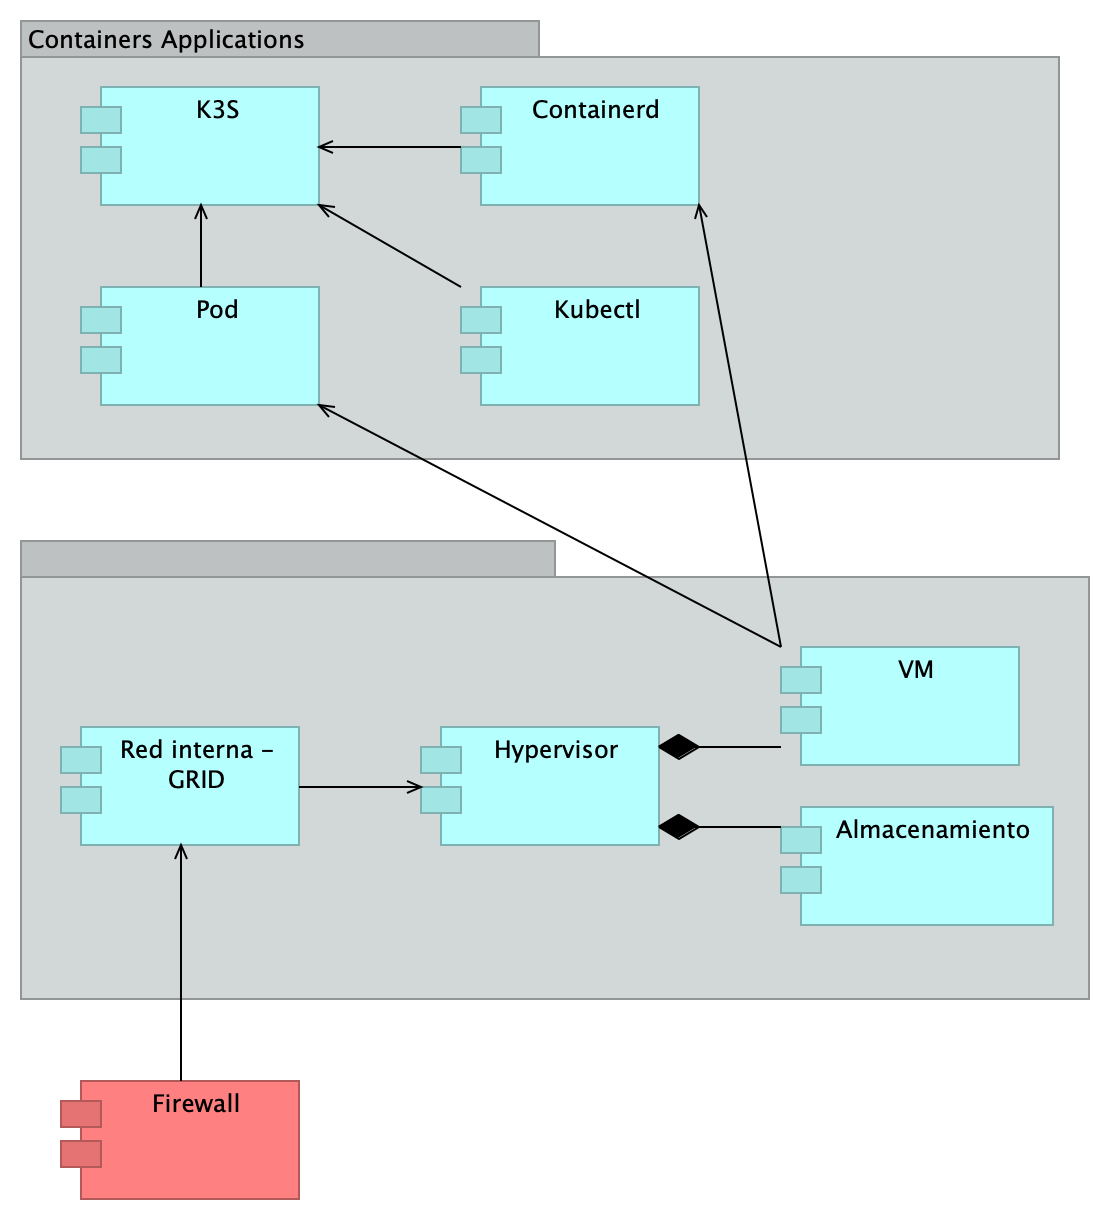
\includegraphics[scale=0.2]{tablas-images/cp6/Application-Cooperation-View.png}
    \caption{Vista de Cooperación de Aplicaciones}\label{fig:vista-cooperacion-aplicacion}
\end{figure}
\noindent
La figura~\ref{fig:vista-comportamiento-aplicacion} presenta la vista de comportamiento de aplicaciones, donde se describe el flujo de actividades relacionadas con la creación automatizada de máquinas virtuales sobre el hipervisor. El proceso inicia con la validación de nombres de las \VM, asociado al parámetro de entrada del número de \textit{workers}, y continúa con la creación del servidor \NAT\ y FailoverNAT, en pro de ofrecer redundancia en la red. Posteriormente, se lleva a cabo la creación de los nodos \textit{master} y \textit{workers}, utilizando como insumo las llaves \SSH\ para la autenticación segura. Finalmente, se realiza la configuración de red, en la cual se definen las direcciones \IP\ y las direcciones \MAC\ de cada nodo. Este comportamiento está agrupado bajo la política de automatización Policy Creation, que organiza de manera estructurada la secuencia de tareas que componen el servicio de creación de \VM, evidenciando cómo los recursos de red, seguridad y cómputo se coordinan para desplegar entornos virtualizados de forma eficiente.
\begin{figure}[H]
    \centering
    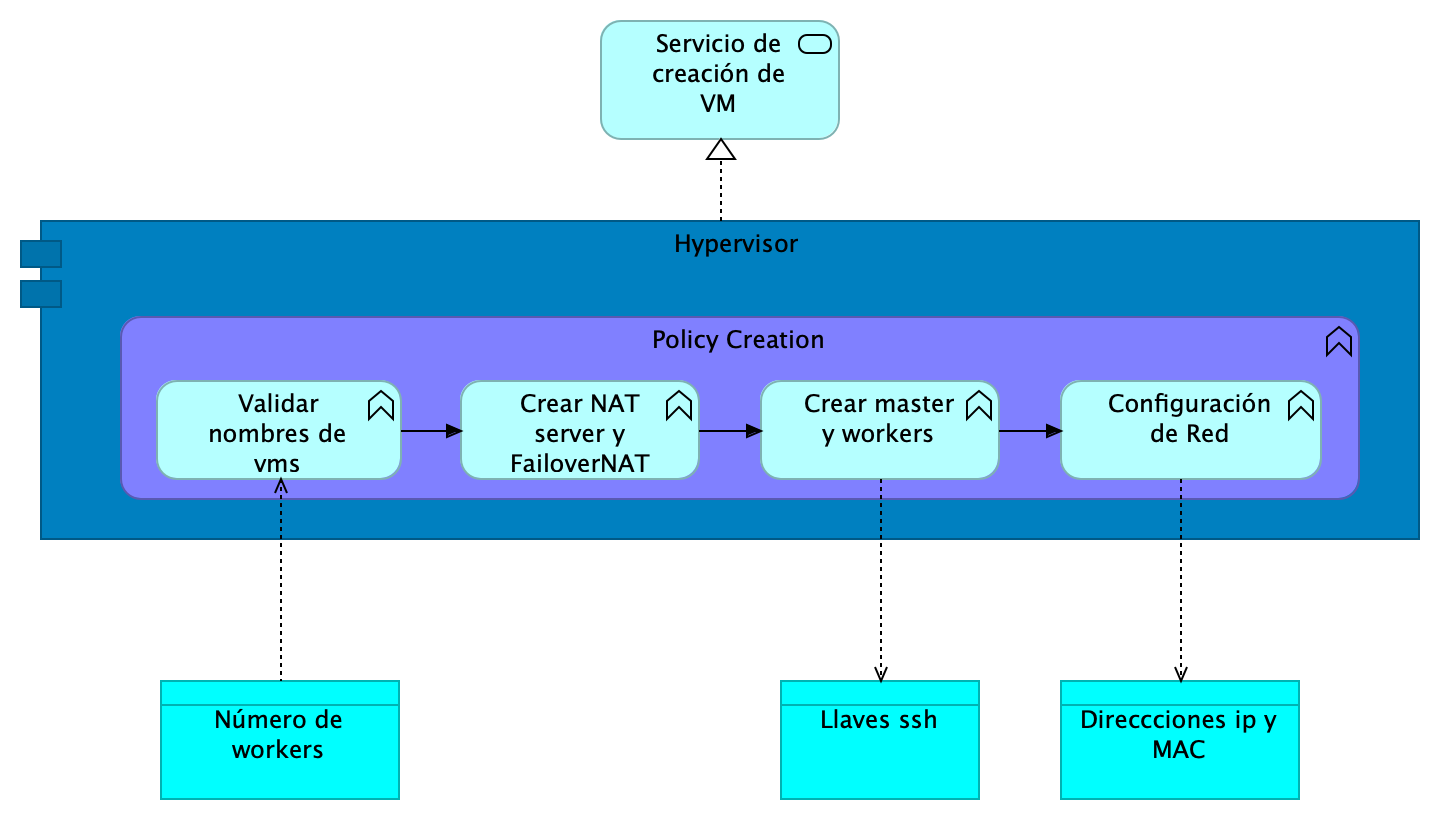
\includegraphics[width=\textwidth]{tablas-images/cp6/Application-Behaviour-view.png}
    \caption{Vista de Comportamiento de Aplicaciones}\label{fig:vista-comportamiento-aplicacion}
\end{figure}
\noindent
El diagrama~\ref{fig:vista-estructura-aplicacion} constituye una vista de estructura de aplicaciones en la cual se modela la organización funcional del sistema de Administración de Recursos del \GRID. En la capa de aplicación, se identifican distintos \textit{Application Components} —como Evaluación de Recursos, Acceso de Investigadores, Gestión de Ejecuciones y Gestión de Entornos Virtualizados— que representan las funcionalidades principales encargadas de articular los procesos del sistema. De este modo, la vista refleja la manera en que los servicios de aplicación soportan la administración de recursos computacionales en el \GRID\ mediante la gestión y persistencia de datos estructurados, buscando la integración entre usuarios, ejecuciones y entornos virtualizados.
\begin{figure}[H]
    \centering
    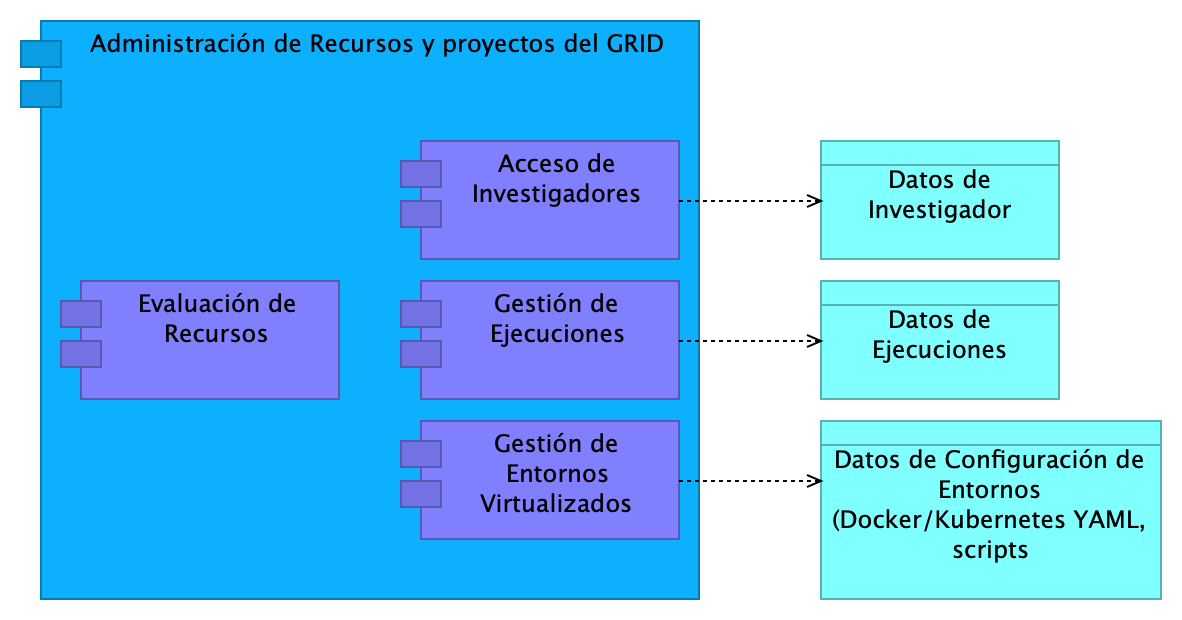
\includegraphics[width=\textwidth]{tablas-images/cp6/Application-Structure-View.png}
    \caption{Vista de Estructura de Aplicaciones}\label{fig:vista-estructura-aplicacion}
\end{figure}